\documentclass[11.5pt]{sig-alternate} % sets document style to sig-alternate
% packages
% typesetting
%\usepackage{dirtytalk} % typset quotations easier (\say{stuff})
\usepackage{hanging} % hanging paragraphs
\usepackage[defaultlines=3,all]{nowidow} % avoid widows
\usepackage[pdfpagelabels=false]{hyperref} % produce hypertext links, includes backref and nameref
\usepackage{xurl} % defines url linebreaks, loads url package
\usepackage{microtype}
% layout
%\usepackage{enumitem} % control layout of itemize, enumerate, description
\usepackage{fancyhdr} % control page headers and footers
\usepackage{float} % improved interface for floating objects
%\usepackage{multicol} % intermix single and multiple column pages
% language
\usepackage[utf8]{inputenc} % accept different input encodings
\usepackage[english]{babel} % multilanguage support
% misc
\usepackage{graphicx} % builds upon graphics package, \includegraphics
%\usepackage{lastpage} % reference number of pages
%\usepackage{comment} % exclude portions of text (?)
\usepackage{xcolor} % color extensions
\usepackage[backend=biber, style=apa]{biblatex} % sophisticated bibliographies % necessary for HTML to display author info and date on abstract page
\usepackage{csquotes} % advanced quotations, makes biblatex happy
\usepackage{authblk} % support for footnote style author/affiliation
% tables and figures
\usepackage{tabularray}
%\usepackage{array} % extend array and tabular environments
\usepackage{caption} % customize captions in figures and tables (rotating captions, sideways captions, etc)
%\usepackage{cuted} % allow mixing of \onecolumn and \twocolumn on same page
\usepackage{multirow} % create tabular cells spanning multiple rows
%\usepackage{subfigure} % deprecated, support for manipulation of small figures
%\usepackage{tabularx} % extension of tabular with column designator "x", creates paragraph-like column whose width automatically expands
%\usepackage{wrapfig} % allows figures or tables to have text wrapped around them
%\usepackage{booktabs} % better rules
% dummy text
%\usepackage{blindtext} % blind text dummy text
%\usepackage{kantlipsum} % Kant style dummy text
%\usepackage{lipsum} %lorem ipsum dummy text
% other helpful packages may be booktabs, longtable, longtabu, microtype

\pagestyle{fancy} % sets pagestyle to fancy for fancy headers and footers

% header and footer
% modern way to set header image
\renewcommand{\headrulewidth}{0pt} % defines thickness of line under header
\renewcommand{\footrulewidth}{0pt} % defines thickness of line above header
\setlength\headheight{80.0pt} % sets height between top margin and header image, effectively moves page contents down
\addtolength{\textheight}{-80.0pt} % seems to affect the lower height. maybe only works properly if footer numbers enabled?
\fancyhf{}
\fancyhead[CE, CO]{
\includegraphics[width=\textwidth]{headerImage.png}}
% footer
%\fancyfoot[LE,LO]{Article Title Here \\ DOI: }% left footer article title and doi
%\fancyfoot[CE,CO]{{}} % center footer empty
%\fancyfoot[RE,RO]{\thepage} % right footer page numbers
%\pagenumbering{arabic} % arabic (1, 2, 3) numbering in footer

\hypersetup{colorlinks=true,urlcolor=blue} % sets link color to blue
\urlstyle{same} % sets url typeface to same as rest of text

% set caption and figure to italics, label bold, left align captions, does not transfer to HTML
\DeclareCaptionFormat{custom}
{
    \textbf{\textit{\large #1#2}}\textit{\large #3} % #1 is the "Table 1" or "Figure 1" part, #2 is the separator (":"), #3 is the caption
}
\captionsetup{format=custom}
\captionsetup{justification = raggedright, singlelinecheck = false}
 
\let\oldabstract\abstract
\let\oldendabstract\endabstract
\makeatletter
\renewenvironment{abstract}
{\renewenvironment{quotation}%
               {\list{}{\addtolength{\leftmargin}{1em} % change this value to add or remove length to the the default
                        \listparindent 1.5em%
                        \itemindent    \listparindent%
                        \rightmargin   \leftmargin%
                        \parsep        \z@ \@plus\p@}%
                \item\relax}%
               {\endlist}%
\oldabstract}
{\oldendabstract}
\makeatother

\begin{document}

\title{Teaching Cybersecurity to Students with Visual Impairments and Blindness}

\author[1]{\large \color{blue}Jesse R. Hairston}
\author[1]{\large \color{blue}Tania Williams}
\author[1]{\large \color{blue}Derrick W. Smith}
\author[1]{\large \color{blue}William T. Sabados}
\author[1]{\large \color{blue}Steven Forney}
\affil[1]{The University of Alabama in Huntsville}

\toappear{}
%% ABSTRACT
\maketitle
\begin{@twocolumnfalse} 
\begin{abstract}
\item 
\textit {This work showcases specific adaptations used to make cybersecurity accessible to high school students with visual impairments and blindness (VIB). The rapidly growing field of cybersecurity demands a diverse workforce; however, barriers exist which can deter students with disabilities from studying cybersecurity, let alone pursuing a career in the field. To help overcome this challenge, we launched the first GenCyber camp specifically developed and instructed for high school students with VIB in summer 2019. We created a unique learning environment by combining inter-active instructional aids, accessible development environments, and innovative instructional strategies. With intent to show cybersecurity as a viable career option for a diverse workforce, the program outcomes from this work included a clear understanding of the GenCyber Cybersecurity Concepts, sparking interest in cybersecurity careers, and building the confidence to pursue those careers. This material is based upon work supported by the National Security Agency and National Science Foundation through the GenCyber program under award number 19-AL-UAHx-UV-S1.}
\\ \\
Keywords: Cybersecurity, Blind, Braille, Visual Impairment, Technology, STEM, Education, Screen Reader, Cryptography, Programming, Escape Room, Sphero Specdrums, Drone, Raspberry Pi
\end{abstract}
\end{@twocolumnfalse}

%% AUTHOR INFORMATION

\textbf{*Corresponding Author, Jesse R. Hairston}\\
\href{mailto: jesse.hairston@uah.edu}{(jesse.hairston@uah.edu)} \\
\textit{Submitted  January 15, 2020}\\
\textit{Accepted February 11, 2020} \\
\textit{Published online February 26, 2020} \\
\textit{DOI:10.14448/jsesd.12.0007} \\
\pagebreak
\clearpage

\begin{large}
\section*{LITERATURE REVIEW}

The field of cybersecurity is one of the fastest growing fields within Science, Technology, Engineering, and Mathematics (STEM) (Information Systems Audit and Control Association [ISACA], 2016). Current estimates state that the field will grow by 32\% within the next 10 years and is projected to be one of the largest fields by 2028 (U.S. Bureau of Labor Statistics, 2019). In response to this growing field, many organizations and universities, including The University of Alabama in Huntsville (UAH), have established degree and training programs directly focused on cybersecurity (LaChance, 2019). While the amount of growth in cybersecurity at this scale could potentially create employment for a diverse workforce, Thurston et al. (2017) report that out of 20\% of all graduate enrollments who disclosed a disability, only 19\% of those were enrolled in programs where science and technology were the focus (3.8\% overall). The gap of students disclosing a disability entering into STEM fields also exists after graduation with only 64\% of STEM graduates with a disability maintaining employment compared to 83\% of those without disabilities.
        	
Individuals with visual impairments and blindness (VIB) are a heterogenous group often struggling to be successful in STEM careers (Antonelli, Steverson, \& O’Mally, 2018). Lack of access to print and graphical information and technological innovations directly related to the field (such as accessible specialized statistical software) serve as the primary challenges for students with VIB to access any STEM career. Due to the difficulty in overcoming these and other challenges, students with VIB are often not introduced to many of the STEM fields in their secondary school experiences (Smith, 2017; Wild \& Koehler, 2017).
        	
Over the past decade, there has been a focused push to provide students with VIB experiences in fields that are desirable but often considered difficult for individuals with VIB. For example, Dr. Andreas Stefik began a camp for teachers of students with VIB to learn how to teach programming using a newly formed accessible programming language called Quorum (Stefik \& Siebert, 2013). Quorum has been taught to hundreds of students with VIB internationally. Lego Mindstorms are popular in STEM activities, but the block-based programming language is not accessible to VIB students. A text-based language, JBrick, has been created to be fully compatible with the JAWS® (Job Access With Speech) screen reader and provides an accessible programming environment to use Lego® Education Mindstorm® materials and even join the Lego® robotics competitions (Ludi, Bernstein, \& Mutch-Jones, 2018). Ludi and her colleagues lead a programming camp for students in coordination with the National Federation of the Blind (NFB) National Center for Blind Youth in Science (NCBYC). The NFB-NCBYC has established multiple STEM camps NFB EQ (Engineering Quotient) with the express purpose to encourage students with VIB to engage in STEM activities. As noted on the NFB’s website, their goal is to empower students to find solutions to access STEM careers (NFB, 2018).

In response to the underrepresentation of individuals with VIB in STEM and the rapidly growing field of cybersecurity, UAH developed and taught the first GenCyber cybersecurity summer camp for high school students with VIB. This article shares lessons learned from the camp experience and provides recommended adaptations for making cybersecurity and other STEM subjects more accessible to students with VIB. This material is based upon work supported by the National Security Agency (NSA) and the National Science Foundation (NSF) through the GenCyber program under award number 19-AL-UAHx-UV-S1.

\section*{ABOUT THE CAMP}

GenCyber is a national program providing cybersecurity summer camp experiences for K-12 students and teachers through funding by the NSA and the NSF. Colleges, universities, and school systems are awarded GenCyber grants to develop and host camps all across the United States. The UAH Center for Cybersecurity Research and Education (CCRE) was awarded the first GenCyber grant to create a cybersecurity camp specifically for high school students with VIB in 2019. The week-long camp curriculum was adapted from proven GenCyber activities for high school students who are deaf and hard-of-hearing and from a pilot specialized transition program for youth with VIB. The curriculum was largely activity- and project-based and steeped in the six GenCyber Concepts: defense in depth, confidentiality, integrity, availability, think like an adversary, and keep it simple. Program outcomes for campers included a clear understanding of the GenCyber Concepts, interest in cybersecurity careers, and confidence to pursue those careers. The CCRE partnered with the Alabama Institute for Deaf and Blind (AIDB) and the Center for Accessible Technology Training, a project collaboration between American Printing House for the Blind and AIDB. Other major partners included Microsoft, the Alabama Department of Rehabilitation Services, and the UAH College of Education.

\section*{ADAPTATIONS}

The camp’s curriculum was comprised of skills generally taught in high school cybersecurity camps. Participants were introduced to ethics, hardware, cryptography, networking, password and online safety, social engineering, computer programming, and digital forensics. All topics were presented in the context of the GenCyber Concepts. The camp’s traditional curriculum was adapted to meet the needs of individuals with VIB and to create an inclusive camp environment. Instructional materials were formatted with larger font size, high contrast color schemes, accessible animations, etc. (Brauner, 2016). Camp materials were offered in digital and braille formats, with students often having a choice of devices, magnification tools, and screen readers. Additionally, the camp made further adaptations in the areas of instructional aides, scheduling and pacing, and instructional strategies and materials.

\subsection*{General Technology Used}

Microsoft® contributed much of the general technology used at camp by loaning UAH a Surface Pro 5 and display adapter for each camper. UAH paired the Surface devices with dedicated monitors, keyboards, and mice. Vispero™, the owners of Freedom Scientific®, provided licenses of the JAWS® and ZoomText® accessibility software. UAH staff pre-installed JAWS®, ZoomText®, and NVDA (NonVisual Desktop Access, an open-source screen reader) on every Surface to ensure campers had access to their preferred accessibility software. Each camper was also provided an Apple® iPad with accessibility features. The first evening of camp was dedicated to campers setting up their devices and any accessibility software or equipment. A DaVinci HD/OCR desktop video magnifier was set up at camp as a station specifically for enhanced magnification and text-to-speech. Prusa 3D printers were used to create learning manipulatives and interactive puzzles. A Picture in a Flash (PIAF) tactile graphic maker with swell-touch paper was used to create tactile graphics for labs and puzzles. A braille labeler was used to make non-digital activities more accessible. Lectures in the classroom were presented on dual projector screens, and campers had digital copies of the lectures converted to a format compatible with screen readers and magnification software.

\subsection*{Instructional Aids}

Instructional aids were used at camp to enhance learning, provide differentiated instruction, and make activities more accessible for campers with VIB. Successfully integrated aids included 3D printed manipulatives, wearable assistive technology, accessible coding environments, and miniature programmable drones.

\textbf{Caesar cipher rings.} The GenCyber Concept of confidentiality has been traditionally introduced at camp by explaining how the Caesar cipher encrypts messages by shifting the alphabet. This lesson is then followed by an activity where campers manually encode and decode messages with the help of 3D printed Caesar cipher rings (Larson, 2011). The original 3D printed rings used for UAH GenCyber camps were small items that would rotate freely and were not accessible to individuals with VIB. Two-dimensional paper Caesar cipher wheels and sticks were successfully prototyped in 2018 with large print, high contrast, and braille (Martin, 2019). The UAH team was able to build on this success by incorporating these characteristics into enhanced 3D printed Caesar cipher rings. Initial prototype rings were made high contrast by printing the entire ring in yellow and using puff paint to manually fill-in black letters; however, this process was tedious and inaccurate. The enhanced rings were remixed from a design that requires slight force to rotate the alphabet each letter, making the rings tactile and easier to manipulate (Fields, 2017). To customize this design, Autodesk’s Inventor Computer Aided Drafting (CAD) program was used to design the enhanced Caesar cipher rings (Inventor, 2019). The new design was achieved by creating the ring using the revolving tool that then cuts with a 26-sided polygon from the top in order to create a character on each polygon side around the ring. The high contrast version was created using a Prusa i3 MK3S 3D printer with a multi material upgrade capable of printing both yellow and black color plastics simultaneously (see Figure 1) (Forney, 2019b). Braille rings were created by braille standard specifications (see Figure 2) (Braille Authority of North America, 2009; Forney, 2019a).

\begin{figure}[ht]
    \centering
    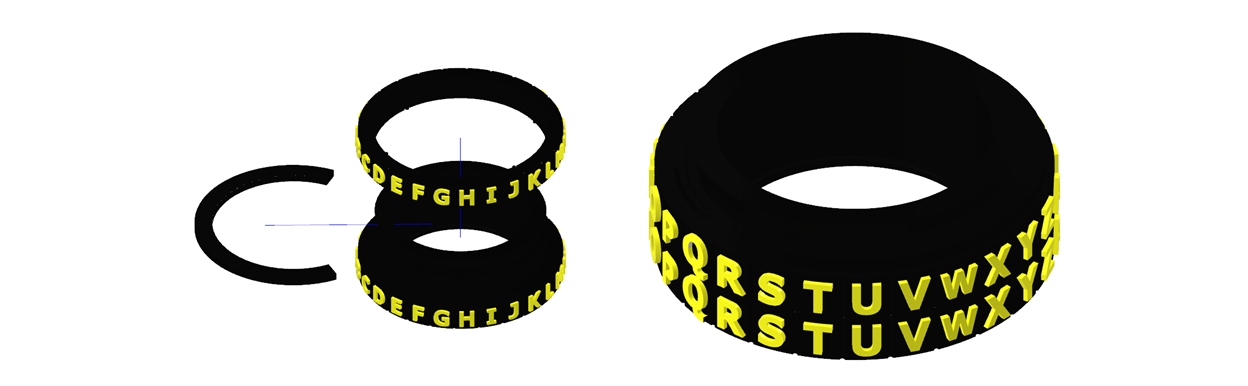
\includegraphics[width=1\linewidth]{1117_Fig1.png}
    \caption{High contrast Caesar cipher ring with tactile feedback. The ring, comprised of two rows of enlarged, yellow letters from the English alphabet, would click when the top row was shifted.}
\end{figure}

\begin{figure}[ht]
    \centering
    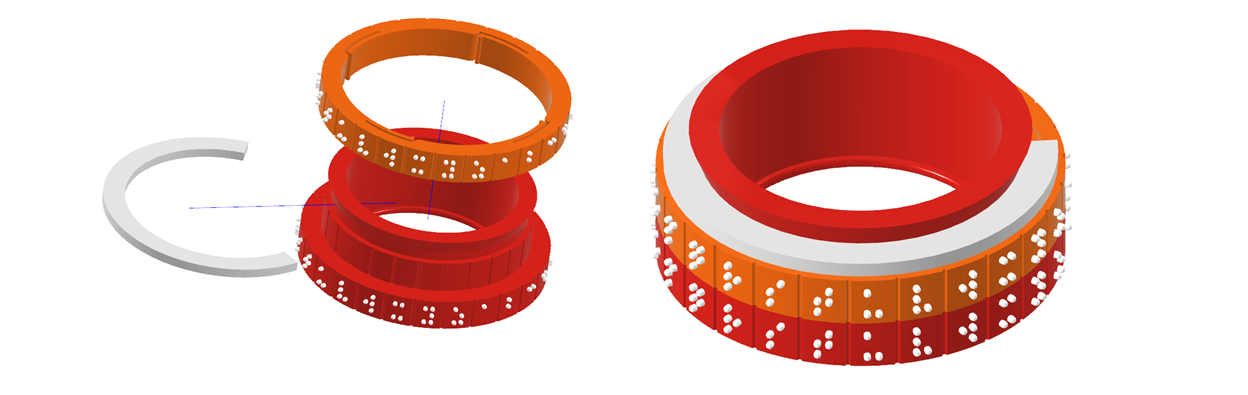
\includegraphics[width=1\linewidth]{1117_Fig2.png}
    \caption{High contrast braille Caesar cipher ring with tactile feedback and two rows of the braille alphabet. The braille cipher ring clicked and offered tactile feedback when the user shifted one of the two rows.}
\end{figure}

\textbf{Wearable assistive technology.} Sphero Specdrums® are bluetooth-enabled rings with color sensors that activate when the ring is tapped against a surface. The Sphero rings pair to devices like iPads where they can map to sounds or custom recordings. Although originally designed for creating music, the rings have been used for accessible learning (Greenhalgh, 2019). Through a collaboration with a teacher from UAH’s GenCyber teacher camp, we developed an activity allowing participants to independently identify the main parts of a computer using these rings (Chamberlain, 2019). Desktop computers were disassembled, and then colored fabric was attached to the main components (e.g. blue attached to the motherboard, green attached to the hard drive). The Sphero software was then used to map the colors to custom audio recordings corresponding to the computer component name (e.g. blue would be mapped to an audio recording of the word motherboard). The desktop computers were then reassembled. Campers participating in the activity would disassemble the desktop computers, feel for the textured fabric, and tap the Sphero rings on the fabric to trigger an audio recording of the computer part’s name. While our campers enjoyed the independence of this activity, the rings were sometimes cumbersome to use and the Sphero software did not reliably save the custom audio mappings to the iPad app.

\textbf{Programming environment.} Programming is a core component of UAH’s cybersecurity camps and is used to convey multiple GenCyber Concepts. Computer programming can be a challenge for people with VIB due to Integrated Development Environments (IDE) not being compatible with screen readers. Also, some programming languages’ syntax and symbols are not conducive to being read aloud (Stefik, Haywood, Mansoor, Dunda, \& Garcia, 2009). We selected the Quorum programming language to help camp participants with no previous programming experience, since it was originally developed with individuals with VIB in mind and has a custom-built SODBeans IDE based on NetBeans that is screen reader friendly (Stefik, Hundhausen, \& Smith, 2011). Prior to camp, the UAH team met with the creator of Quorum and enlisted the aid of an experienced Quorum instructor to get advice on how to tailor our camp’s programming curriculum. The major insight was to allocate more time for campers to customize their IDE and gain familiarity with how it functions. Quorum served as a good starting point for beginner programmers, but campers with prior programming experience expressed a desire to work with more mainstream, and thus, more marketable programming languages.

\textbf{Drone programming.} In addition to Quorum-based programming labs, the camp included drone-based programming activities. Drone programming has proven to be a popular camp activity in the past because it allows participants to manipulate and play with a physical object, a drone, while reinforcing the algorithmic thinking that was introduced in our previous programming labs. For our campers with VIB, we selected the Swift Playgrounds app as the drone-based development environment because of its accessibility support using the iPad’s magnification and VoiceOver features. At first, we were not sure how drone programming would be received by the participants, but it proved to be a very successful activity. One student was even able to connect her refreshable braille display to the iPad and program the drone. The drones made enough noise in flight that participants with VIB were able to follow successful maneuvers. 

\subsection*{Instructional Strategies/Materials}

While the skills taught in GenCyber were consistent with those taught in other cybersecurity camps, the instructional approaches differed. For instance, to commemorate the camp being the first GenCyber camp specifically for individuals with VIB, the camp t-shirt included a cipher that was dependent upon the braille alphabet to decipher. Additionally, while cryptography and steganography (the process of hiding messages within pictures) are traditionally tied to visuals, the labs, instead, utilized sound. Cryptography was taught using the example of the Navajo code used in World War II, which is a spoken form of cryptography (Code Talking). Instead of embedding messages in pictures for steganography, the labs centered around messages hidden in music. These adaptations also included the way we assessed participants. In order to assess camper performance, review activities were included in the form of scavenger hunts, escape room type challenges, and exit tickets. 

\textbf{Scheduling, orientation, and pacing.} Ganesh and Narendran (2018) note that individuals with VIB often lack the opportunities for incidental learning and need more time to explore their learning environments and complete assignments. As such, camp schedules were adapted to include time for orientation and slower instructional pacing. Beginning on the first day of camp, campers were given time to become familiar with their workstations and to set up their assistive technology. Experts were on hand to help with this and offer additional assistance throughout the camp. Instructors provided more transition time between tasks and offered time during the day for campers to explore special topics in small groups, review, or finish labs from earlier in the day. 

\textbf{Scavenger hunt.} The scavenger hunt activity was designed as a formative assessment to gauge content learned while reinforcing problem-solving skills and collaboration (Ramsey, 2018, p. 155). The activity was based on an existing game developed by Norwich University staff (Read, Mattrick, Pessolano, 2016), where campers used a Wi-Fi analyzer to track down Raspberry Pi devices acting as rogue access points. In the original activity, the campers used mobile devices installed with the Farproc Wifi Analyzer Android app to find the hidden Raspberry Pis and, after finding a Raspberry Pi, would access a webpage hosted on the Raspberry Pi utilizing a WiFi network name and password attached to the devices (Farproc). The webpage corresponding to the Raspberry Pi would pose a review question. If the team answered the question correctly, it would be provided with a clue. The first team to collect all the clues would win the hunt.

While the Farproc tool offered the option in the application to track the proximity of the devices by a series of beeping sounds, we were concerned that camp participants would have difficulty associating the beeps with a specific device. Instead, we fitted each device to emit its own unique song using a buzzer. For example, one hidden device might play the Tetris theme, while another might play a few lines from a Star Wars song. Campers could listen for the unique sound assigned to each device to assist with finding each clue. The activity was further adapted through the use of braille. When the campers located the Raspberry Pi, the login information to access the review questions was also in braille and attached to the devices. From this point, the campers would still log into the devices and answer the review question to obtain the clue. 

\textbf{ESCaPE zones.} Additionally, researchers utilized problem-solving challenges to reinforce skills taught in camp. Some of these challenges were in the form of daily review exercises called Engaging Students in Cybersecurity and Programming Education (ESCaPE) Zones (Hairston \& Williams, 2019). These zones offered activities mimicking a traditional escape room but were developed to assess skills specific to camp. The ESCaPE Zones were used three times during camp, with the last activity being a review of all previous days. 

\textbf{\textit{ESCaPE Zone 1.}} The first ESCaPE Zone reviewed the concept of confidentiality by requiring campers to decode a Cardan grille cipher and a Caesar cipher, skills they were taught previously. Here, campers were given a lockbox, secured with a directional padlock. In order to find the combination for the lock, campers utilized a Cardan grille cipher (Spycraft). The Cardan grille cipher comprised of a page of arrows, pointing in various directions, raised using a PIAF machine. A corresponding 3D printed Cardan grille had rectangle-shaped holes which would reveal the directional combination to the padlock when it was oriented correctly over the page of arrows (see Figures 3 and 4). After using this tactile key to gain access to the lockbox, campers found a message encoded with a Caesar cipher and the 3D printed cipher rings mentioned earlier. Participants utilized the cipher rings to decode the message, which was a review question. Answering the review question correctly was the end of that ESCaPE challenge.

\begin{figure}[ht]
    \centering
    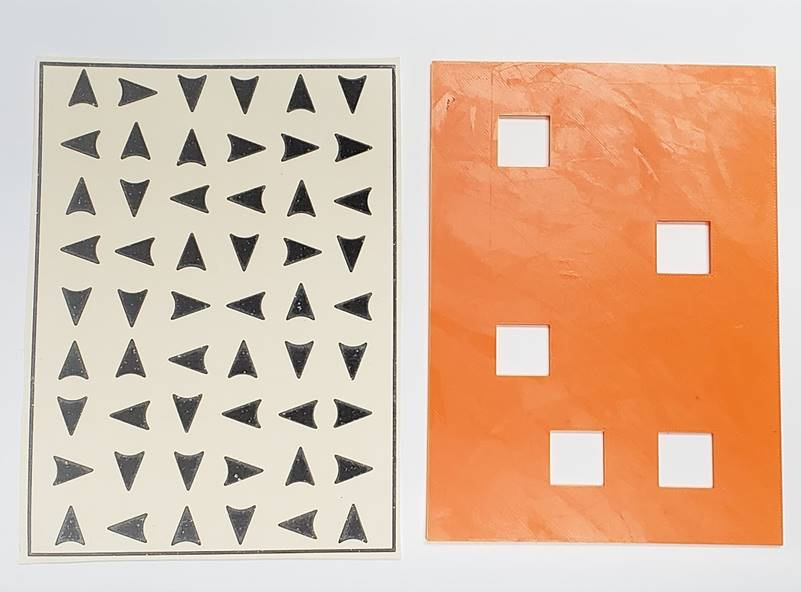
\includegraphics[width=1\linewidth]{1117_Fig3.jpg}
    \caption{Example of a Cardan grille cipher with corresponding grille. The 9 rows of 6 arrows pointing in various directions were first printed using black ink on swell-touch paper. The arrows were raised when the paper was processed through a PIAF machine, allowing a tactile representation of the cipher (see left). The 3D printed grille (shown right) served as the key for the cipher.}
\end{figure}

\begin{figure}[ht]
    \centering
    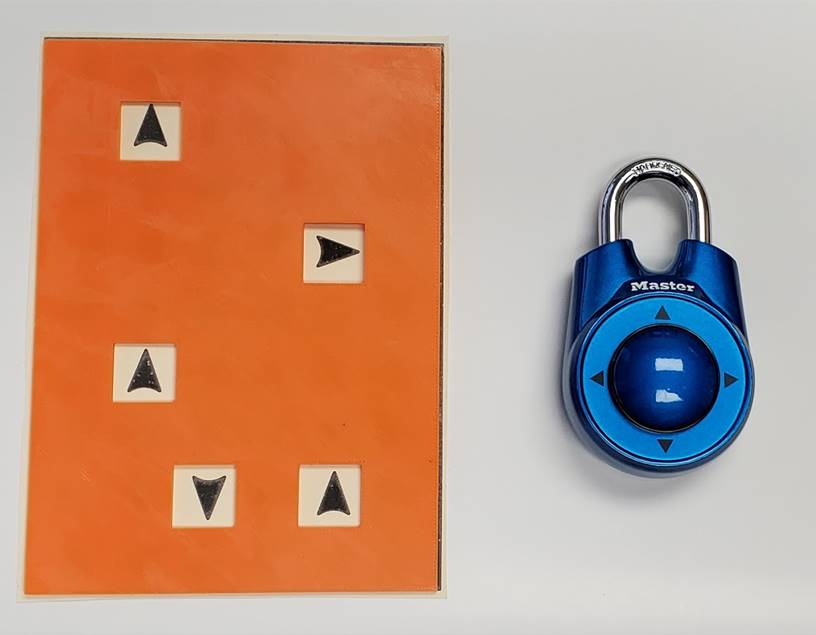
\includegraphics[width=1\linewidth]{1117_Fig4.jpg}
    \caption{Example of a solved Cardan grille cipher and corresponding directional lock. When the 3D printed grille was turned properly and placed over the arrows, the correct combination to open the directional lock was revealed (shown left). This combination could then be used to open a directional lock like the one pictured (shown right).}
\end{figure}

\textbf{\textit{ESCaPE Zone 2.}} The second ESCaPE Zone reviewed social engineering and networking. This activity began by placing a locked metal box at the front of the room with a unique design of a key drawn on top (see Figure 5). The key design is known as Warchalking, the art of drawing special symbols in public areas to indicate types of WiFi networks. The design was projected in the classroom using a document camera. Additionally, a tactile printout of the shape, created using a PIAF machine, was provided to each group of campers. A Twitter profile URL was given to the campers, and they were instructed to use the website to discover the mystery of the locked metal box. The Twitter profile was populated with posts containing a mixture of puzzles to further progress in the ESCaPE Zone and red herrings which offered no progress. Some posts contained pictures with descriptive alternative text to ensure accessibility with screen readers. To complete the review activity, campers had to investigate the Twitter page, discover the symbol on the locked metal box denotes a WiFi access point, and discern the metal box contained a Raspberry Pi device broadcasting its own WiFi signal. Campers needed to find a password hidden on the webpage to connect to the Raspberry Pi WiFi device. Successfully connecting revealed a webpage with a review question about steganography. Entering the correct answer provided campers the GPS coordinates to a location and concluded the ESCaPE Zone.

\begin{figure}[ht]
    \centering
    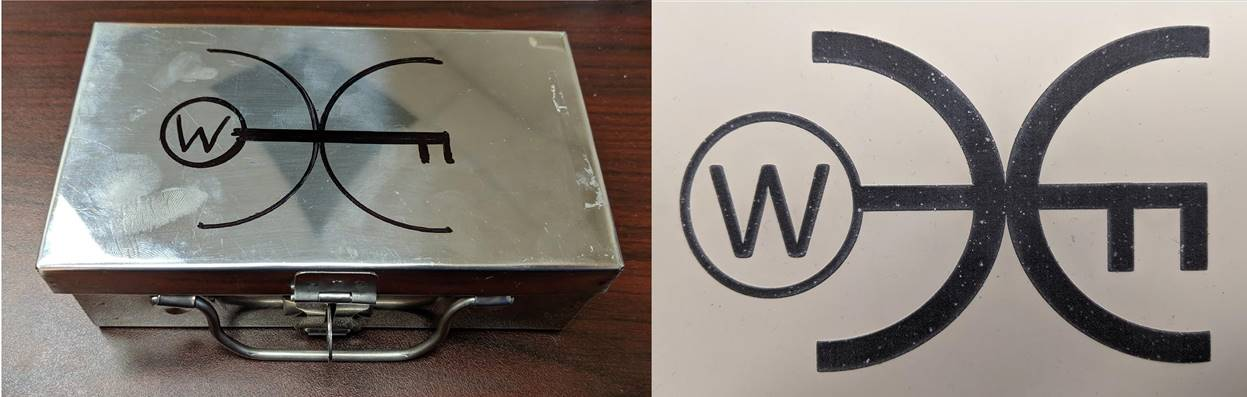
\includegraphics[width=1\linewidth]{1117_Fig5.jpg}
    \caption{A metal box containing a Raspberry Pi broadcasting a WiFi network. A drawing of a symbol of a key with a ‘W’ in its handle and two half circles (shown left). A tactile graphic of the same key symbol created using a PIAF machine and swell-touch paper (shown right) were used to denote a WiFi access point.}
\end{figure}

\textbf{\textit{ESCaPE Zone 3}}. On the final day of camp, the ESCaPE Zone was a review of skills taught throughout the week. These consisted of three different challenges: hardware assembly, password safety, and cryptography. Challenge one involved participants working in groups to disassemble a desktop computer. A piece of paper with a review question in braille was hidden underneath the motherboard. The question related to the function of a hardware component. By disassembling the computer and answering the question correctly, participants were able to demonstrate their understanding of the parts of a computer.

Challenge two assessed the campers’ knowledge of social engineering and password safety. In this challenge, the campers were given an encrypted ZIP file and some audio files on a device. Campers had to play the audio files to guess the password to open the ZIP file. The ZIP file had another review question inside of it that participants had to answer before going on to the next challenge.

The third challenge reinforced the campers’ problem solving and cryptography skills. Instructors presented participants with a puzzle box (3DPRINTINGWORLD, 2018). Once opened, the participants found Caesar cipher rings like the ones discussed above and an encrypted message in braille. The decoded message was a review question related to cryptography the campers had to answer correctly to complete the challenge. 

\textbf{\textit{Exit tickets}}. Finally, learning was assessed through the use of exit tickets. At the close of the day’s lesson, groups of campers were given a Sphero Specdrums® ring. They walked to an area of the room where a question and corresponding colored square was posted on the wall. Campers used the ring to tap on the colored square, where they could listen to a recording of the review question using an iPad. Students were encouraged to discuss their thoughts as a group and record their responses on the poster or report their answers to a staff member to record.

\section*{HUMAN CAPITAL}

Perhaps the most important aspect of our camp was its use of human capital. Human capital, which leverages “the whole set of human knowledge, skills, abilities, and motivations,” makes use of professional experience to achieve growth (Azatovna, 2109, p. 411). In the case of camp, the staff sought to maximize its organizational structure to best utilize the camp’s intellectual resources. This structure included the way students were grouped, the use of mentors and guest speakers, and the allocation of camp staff.

\subsection*{Groups}

To encourage collaboration and social interaction, staff arranged campers in cooperative groups (Ward, 1987). The teams consisted of three to four individuals each, with the campers seated at round tables organized in the classroom area. These teams were diverse, heterogeneous groupings, with participants of similar ranges of vision spread across the room. The instructors also made efforts to ensure each group had representatives from different ages and geographic locations and had equal gender representation. This strategy created a balance among the groups for competitions, allowed campers to meet new people, and encouraged participants to help each other.

In addition to these static team groupings, flexible groups were used for a time period after lunch each day when campers were given the choice of small group instruction from a list of topics or could use the time to catch up or explore areas individually.

\subsection*{Mentors}

Each group was assigned a near peer mentor. These mentors were college students employed by the camp partners who facilitated group discussions, provided assistance with lab assignments, and helped campers with orientation and mobility. These mentors also advised instructors about pacing and alerted instructors to any other problems relating to the teams.

\subsection*{Guest Speakers}

Guest speakers were also a vital component of camp. Four speakers were recruited for camp, each having a unique message for the campers. The first speaker was an expert from Microsoft who discussed with campers the company’s accessibility tools and its hiring programs. The Federal Bureau of Investigation (FBI) provided an agent to speak to the need for cybersecurity professionals and to the inclusiveness of that organization. An owner of an assistive technology company provided his experience as an individual with VIB who found success in the field of technology. Additionally, a representative from the university's disability support services provided campers with information about advocating for their needs as university students.

\subsection*{Camp Staff}
 
 The camp staff was also diverse. The curriculum developers served as instructors and came from a wide range of backgrounds. Seasoned educators worked with content area experts to develop instructional content and strategies. Additionally, the camp made use of college students training to become Teachers of Students with Visual Impairments (TVIs).

\textbf{Instructional developers.} Curriculum developers came from a wide range of disciplines, including education, assistive technology, computer engineering, computer science, information systems, and electrical and mechanical engineering. We enlisted the aid of Jill Dunaway, a proficient Quorum instructor and assistive technology teacher from the Alabama School for the Blind who is also an individual with VIB. Jill assisted with teaching Quorum at camp, provided assistive technology support, and reviewed curriculum to ensure accessibility. Steven Forney, a Deaf researcher at UAH and STEM professional, also joined the team to offer his expertise using CAD software, printing 3D manipulatives, and providing support for drone activities. As mentioned earlier, near peer mentors provided campers with role models close to their own age. 

\textbf{TVIs.} The College of Education at UAH has a graduate program that trains educators to become TVIs. Five UAH TVI graduate students supported the camp experience as part of their mandatory practicum. During the week, the graduate students provided overall support for the camp including supporting basic orientation and mobility (O\&M), assistive technology support, curriculum support, and behavior monitoring. From a practical vantage, the experience allowed the graduate students to work with “high-functioning, college-bound” students. There were also two graduate students with visual impairments themselves and four of the five teachers were already hired as TVIs at either the Alabama School for the Blind or the Helen Keller School of Alabama. 

\section*{FUTURE DIRECTIONS}

While these adaptations were overall a success, we believe sharing encountered challenges would also be helpful in mitigating pitfalls in future programs. The challenges we faced dealt primarily with training, technology, tool and website compatibility, workbook distribution, and transition time. 

A great deal of staff training is recommended both in terms of the primary subject area (cybersecurity in this case) and the assistive technology. Since this camp experience was high technology, it was apparent a single subject matter expert for a given technology, such as Quorum and its SODBeans IDE, would be a bottleneck, and thus we recommend cross-training staff. Many cybersecurity tools and websites we reviewed did have compatibility issues with screen readers. We recommend reviewing these resources far in advance of the planned activity and promoting the development of accessible environments and interfaces for individuals with VIB. We solely used a digital workbook for our camp; however, if resources allow, we also recommend offering the option of large print and braille copies of a physical workbook. A digital workbook may be enhanced by formatting it for compatibility with screen readers, taking advantage of headers, alternative text, etc. Adequate transition time should be given to participants to ensure they can orient themselves when changing to a new activity or area. Additionally, we plan to review other technologies to supplement future iterations of this camp, including bone conducting headphones, physical programming manipulatives, and hands-free magnification.

\section*{CONCLUSION}

The GenCyber camp for high school students with VIB had the ultimate goals of conveying a clear understanding of the GenCyber Concepts, increasing interest in cybersecurity careers, and growing confidence to pursue those careers. This new camp concept required the development of accessible activities to teach cybersecurity to individuals with VIB. 

Many of the existing tactics and resources presented in this article are the result of work by researchers and educators to advance the accessibility of STEM. These tactics were modified and applied to the topic of cybersecurity to create an interactive, educational environment. Many activities were pilot developments, and we plan to create more cybersecurity activities developed at their origin to be accessible by individuals with VIB. This will consequently open up the rapidly growing field of cybersecurity to diverse professionals who will bring new perspectives and skills to the table.

\section*{ACKNOWLEDGEMENTS}

Funding for this project was supported by the National Security Agency and National Science Foundation through the GenCyber program under award number 19-AL-UAHx-UV-S1. The Alabama Institute for Deaf and Blind and Center for Accessible Technology Training provided student transportation to camp and camper supervision. Microsoft provided much of the technology at camp and a guest speaker. The Alabama Department of Rehabilitation Services provided staff support. We would also like to thank Anna Rodgers for providing support for the project as well as language editing and proofreading for this article. 

\end{large}
\include{} 
\section*{REFERENCES}\par 

\begin{hangparas}{0.25in}{1}

3DPRINTINGWORLD. (2018, July 8). Secret Butterfly Box. Retrieved January 7, 2020, from \url{https://www.thingiverse.com/thing:2977908}

Antonelli, K., Steverson, A., \& O’Mally, J. (2018). College graduates with visual impairments: A report on seeking and finding employment. \textit{Journal of Visual Impairments \& Blindness, 112}(1), 431-443.

Azatovna Galiakberova, A. (2019). Conceptual analysis of education role in economics: The Human Capital Theory. \textit{Journal of History, Culture \& Art Research / Tarih Kültür ve Sanat Arastirmalari Dergisi, 8}(3), 410–421. \url{https://doi-org.elib.uah.edu/10.7596/taksad.v8i3.2256}

Braille Authority of North America. (2009). \textit{Size and spacing of braille characters} [PDF file]. Retrieved from \url{http://www.brailleauthority.org/sizespacingofbraille/sizespacingofbraille.pdf}

Brauner, D. (2016, October 3). Creating accessible PowerPoint presentations for students with visual impairments and blindness. Retrieved January 7, 2020, from \url{https://www.perkinselearning.org/technology/digital-transitions/creating-accessible-powerpoint-presentations-students-visual}.

Chamberlain, April. (2019, June 19). Personal interview.

Code Talking: Intelligence and bravery. (n.d.). Retrieved January 8, 2020, from \url{https://americanindian.si.edu/education/codetalkers/html/chapter4.html}.

Farproc. (2018). Wifi Analyzer (3.11.2) [Mobile application software]. Retrieved from \url{https://play.google.com/store/apps/details?id=com.farproc.wifi.analyzer\&hl=en\_US}

Fields, J. (2017, December 11). Cipher ring V4 by osj1961. Retrieved December 19, 2019, from \url{https://www.thingiverse.com/thing:2706672}.

Forney, S. (2019a, August 1). Caesar cipher decoder ring - Braille version. Retrieved December 20, 2019, from https://www.prusaprinters.org/prints/4725-caesar-cipher-decoder-ring-braille-version.

Forney, S. (2019b, August 2). Caesar cipher decoder ring - English alphabet letters. Retrieved December 20, 2019, from \url{https://www.prusaprinters.org/prints/4764-caesar-cipher-decoder-ring-english-alphabet-letter.}

Ganesh, S., \& Narendran, K. (2018). Expert comments on: Are children with low vision adapted to the visual environment in classrooms of mainstream schools? \textit{Indian Journal of Ophthalmology, 66}(2), 290. \url{https://doi-org.elib.uah.edu/10.4103/ijo.IJO\_1315\_17}

Greenhalgh, N. (2019, January 7). Boulder’s Sphero launches musical rings to teach kids coding. Retrieved January 13, 2020, from \url{https://www.americaninno.com/colorado/boulders-sphero-launches-musical-rings-to-teach-kids-coding/}.

Hairston, J. \& Williams, T. (2019, December). A teacher’s ESCaPE Zone. \textit{NICE K12 Cybersecurity Education Conference.} Workshop presented at NICE K12 Cybersecurity Education Conference, Orange County, California. 

Information Systems Audit and Control Association. (2016). Retrieved from \url{https://image-store.slidesharecdn.com/be4eaf1a-eea6-4b97-b36e-b62dfc8dcbae-original.jpeg}

Inventor [Computer software]. (2019). Retrieved from \url{https://www.autodesk.com/products/inventor/overview}

LaChance, D. (2019, January 30). New degree program will help address predicted global shortfall of cybersecurity professionals. Retrieved from \url{https://www.uah.edu/news/campus/new-degree-program-will-help-address-predicted-global-shortfall-of-cybersecurity-professionals}.

Larson, J. (2011, December 21). Caesar cipher decoder ring rounded by cymon. Retrieved December 19, 2019, from \url{https://www.thingiverse.com/thing:14891}.

Ludi, S., Bernstein, D., \& Mutch-Jones, K. (2018). Enhanced robotics!: Improving building and programming learning experiences for students with visual impairments. \textit{ACM Technical Symposium on Computer Science Education,} 372-377. \url{https://doi.org/10.1145/315-9450.3159501}

Martin, Jason. (2019). Teaching basic cryptography concepts using braille and large print manipulatives, \textit{Journal of Science Education for Students with Disabilities: Vol. 22}(1), DOI: 10.14448/jsesd.11.0007 Available at: \url{https://scholarworks.rit.edu/jsesd/vol22/iss1/6}

National Federation of the Blind (NFB) (2018). NFB EQ. Retrieved from \url{https://blindscience.org/nfbeq}.

Ramsey, U. (2018). Americans with Disabilities Act scavenger hunt. \textit{Journal of Legal Studies Education, 35}(1), 143–164. \url{https://doi-org.elib.uah.edu/10.1111/jlse.12072}

Read, H., Mattrick, E., \& Pessolano, G. (2016, September). WiFi treasure hunt. GenCyber Fall Meeting 2016. Boston, MA.

Stefik, A. S., \& Siebert, S. S. (2013). An empirical investigation into programming language syntax. \textit{ACM Transactions on Computing Education, 13}(4), 19:1–19:40.

Smith, D.W. (2017). Mathematics. In M.C. Holbrook, C. Kamei-Hannan, \& T. McCarthy (Eds.), \textit{Foundations of Education} (3rd ed.): \textit{Volume II: Instructional strategies for teaching children and youths with visual impairments.} New York: AFB Press.

Spycraft: The Cardan grille system. (2014, April 13). Retrieved from \url{https://spycurious.wordpress.com/2014/04/13/spycraft-the-cardan-grille-system/}.

Stefik, A., Haywood, A., Mansoor, S., Dunda, B., \& Garcia, D. (2009). SODBeans. \textit{IEEE 17th International Conference on Program Comprehension.} 293-294. \url{https://doi.org/10.1109/ICPC.2009.5090064}

Stefik, A., Hundhausen, C., \& Smith, D. (2011). On the design of an educational infrastructure for the blind and visually impaired in computer science. \textit{Proceedings of the 42nd ACM Technical Symposium on Computer Science Education (SIGCSE ’11)}. 571–576. \url{https://doi.org/10.1145/1953163.1953323}

Thurston, L.P., Shuman, C., Middendorf, B.J., \& Johnson, C. (2017). Postsecondary STEM education for students with disabilities: Lessons learned from a decade of NSF funding. \textit{Journal of Postsecondary Education and Disability, 30}(1), 49-60. 

U.S. Bureau of Labor Statistics (2019, September 4). Information Security Analysts. \textit{Occupational Outlook Handbook}. Retrieved from \url{https://www.bls.gov/ooh/computer-and-information-technology/information-security-analysts.htm}

Ward, Beatrice A. (1987). Instructional groupings in the classroom. \textit{School Improvement Series: Research You Can Use}. Retrieved from \url{https://www.google.com/url?sa=t\&rct=j\&q=\&esrc=s\&source=web\&cd=1\&cad=rja\&uact=8\&ved=2ahUKEwiZwZOqu_LmAhWImeAKHX0xCUkQFjAAegQIARAC\&url=https\%3A\%2F\%2Feducationnorthwest.org\%2Fsites\%2Fdefault\%2Ffiles\%2FInstructionalGrouping.pdf\&usg=AOvVaw1QCgmIXtUT_FtYCCWAhche} 

Wild, T.A., \& Koehler, K.E. (2017). Science. In M.C. Holbrook, C. Kamei-Hannan, \& T. McCarthy (Eds.), \textit{Foundations of Education} (3rd ed.): \textit{Volume II: Instructional strategies for teaching children and youths with visual impairments}. New York: AFB Press.

\end{hangparas}
\end{document}
